% LaTeX skeleton for cs.LG submission
\documentclass[11pt]{article}
\usepackage[utf8]{inputenc}
\usepackage{amsmath,amssymb}
\usepackage{graphicx}
\usepackage{tikz}
\usepackage{booktabs}
\usepackage{microtype}
\usepackage{hyperref}
\usepackage[numbers]{natbib}
\usepackage{geometry}
\geometry{margin=1in}

\title{Temporal Neuro-Symbolic Joint Telemetry State Matrices for Fault-Tolerant Autonomous Navigation}
\author{\textbf{Ayushman Saini} \\ \textit{Independent Researcher} \\ India \\ \texttt{ayushmansaini120@gmail.com}}
\date{June 2026}

\begin{document}
\maketitle
\begin{abstract}
Deep neural networks frequently suffer catastrophic degradation under out-of-distribution (OOD) inputs and corrupted sensor streams. We present a temporal Neuro-Symbolic architecture that couples a high-dimensional neural perception pipeline with a non-parametric differentiable kinematic voting layer. The perception network maps consecutive image frames into motion-aware probabilities; the symbolic layer forms an Einstein-summation outer product that enforces physical consistency and isolates corrupted sensor channels. Evaluated on KITTI-derived temporal pairs, our system attains robust navigation integrity under nominal and extreme multi-channel corruption scenarios. Code and figures are provided with the submission.

\end{abstract}

\section{Introduction}
This work studies a hybrid Neuro-Symbolic design that combines learned perceptual representations with a lightweight, differentiable symbolic layer to achieve graceful degradation under sensor corruption. The central idea is to preserve expressive neural representations for high-dimensional inputs while constraining downstream decisions with exact kinematic relationships implemented as a deterministic voting mechanism. We motivate this architecture by the failure modes observed when deep models are exposed to OOD sensor perturbations and show how structural inductive biases can be used to protect safety-critical telemetry.


\section{Related Work}
We position this work at the intersection of robust machine learning, sensor fusion, and neuro-symbolic integration. Traditional probabilistic filtering approaches (e.g., Kalman filtering) provide principled state estimation for low-dimensional telemetry but do not operate directly on raw images \cite{kalman1960new,thrun2005probabilistic}. End-to-end deep sensor-fusion models can learn rich representations but are vulnerable to out-of-distribution (OOD) failures and catastrophic forgetting \cite{goodfellow2016deep}. Neuro-symbolic methods aim to combine the strengths of symbolic reasoning with neural perception; foundational treatments include \cite{garcez2009neural}. Recent work in combining deep learning with explicit symbolic constraints has demonstrated improved robustness and interpretability in safety-critical domains. Our contribution extends this paradigm by embedding kinematic constraints directly into the inference pipeline, providing guaranteed consistency even under sensor corruption.


\section{Method}
\subsection{Problem setup}
We consider temporal pairs of sensor observations $(I_t, I_{t+1})$ together with auxiliary odometry readings. Our goal is to estimate a discretized forward motion state $s\in\{1,\dots,K\}$ robustly when one or more sensor streams are corrupted.

\subsection{Perception (System 1)}
The perception module $\mathcal{P}_\theta$ is a convolutional neural network that maps a stacked 6-channel temporal tensor $X_t = [I_t, I_{t+1}]$ to a categorical probability vector over speed buckets: $p_{cam}=\mathcal{P}_\theta(X_t)\in\Delta^{K-1}$.

\subsection{Differentiable symbolic voting (System 2)}
We compute a joint voting tensor via an Einstein-summation outer product between independent modality distributions (camera, odometer, speed prior):
$$\mathbf{M}_{i,j,k} = \mathbf{p}_{\text{cam},i}\; \mathbf{p}_{\text{odo},j}\; \mathbf{p}_{\text{speed},k}$$
The isolator evaluates deterministic logical rules over indices of $\mathbf{M}$ (for example, consistency rules that select compatible triples) and reduces $\mathbf{M}$ to an isolated posterior over states. In practice the reduction is implemented as a weighted sum and a small, fixed set of logical masks $\Phi$ that enforce kinematic feasibility.

\subsection{Architecture schematic}
Figure~\ref{fig:arch} depicts the high-level architecture: a temporal image pair enters the perception CNN (System 1) producing a discrete probability vector; auxiliary odometry and a speed prior produce additional categorical distributions; an Einstein-summation outer product forms a joint tensor; deterministic masks $\Phi$ prune inconsistent combinations and produce the final posterior over motion states.

\begin{figure}[!t]
	\centering
	\resizebox{0.98\linewidth}{!}{%
	\begin{tikzpicture}[
		font=\small,
		>=Latex,
		node distance=10mm and 14mm,
		every node/.style={align=center},
		base/.style={draw, thick, rounded corners=4pt, minimum height=1.0cm, text width=3.0cm, inner sep=5pt},
		sensor/.style={base, fill=gray!10, draw=gray!55!black},
		neural/.style={base, fill=blue!8, draw=blue!55!black, text width=3.4cm},
		symbolic/.style={base, fill=orange!10, draw=orange!65!black, text width=3.5cm},
		output/.style={base, fill=green!10, draw=green!50!black, text width=2.7cm},
		arrow/.style={->, thick, draw=gray!70!black}
	]
		\node[sensor] (frames) {6-channel temporal stack\\$[I_t, I_{t+1}]$};
		\node[sensor, below=of frames] (speed) {Speed prior\\$\mathbf{p}_{\text{speed}}$};
		\node[sensor, below=of speed] (odo) {Odometer\\$\mathbf{p}_{\text{odo}}$};

		\node[neural, right=of frames] (cnn) {Perception CNN\\$\mathcal{P}_\theta$\\$\mathbf{p}_{\text{cam}} \in \Delta^{K-1}$};
		\node[symbolic, right=of cnn] (outer) {Tensor outer product\\$\mathbf{M}_{i,j,k} = \mathbf{p}_{\text{cam},i}\,\mathbf{p}_{\text{odo},j}\,\mathbf{p}_{\text{speed},k}$};
		\node[symbolic, right=of outer] (mask) {Symbolic mask ($\Phi$)\\Kinematic rules};
		\node[output, right=of mask] (posterior) {Posterior\\$\mathbf{P}(V=m)$};

		\begin{scope}[on background layer]
			\node[draw=blue!40, dashed, rounded corners=6pt, fill=blue!4, inner sep=10pt, fit=(frames) (cnn), label={[blue!70!black]above:\textbf{System 1: Neural perception}}] {};
			\node[draw=orange!40, dashed, rounded corners=6pt, fill=orange!4, inner sep=10pt, fit=(outer) (mask), label={[orange!70!black]above:\textbf{System 2: Symbolic constraints}}] {};
		\end{scope}

		\draw[arrow] (frames) -- (cnn);
		\draw[arrow] (speed.east) -- node[above, font=\scriptsize] {$\mathbf{p}_{\text{speed}}$} ($(outer.west)+(0,0.25)$);
		\draw[arrow] (odo.east) -- node[below, font=\scriptsize] {$\mathbf{p}_{\text{odo}}$} ($(outer.west)+(0,-0.25)$);
		\draw[arrow] (cnn) -- node[above, font=\scriptsize] {$\mathbf{p}_{\text{cam}}$} (outer);
		\draw[arrow] (outer) -- node[above, font=\scriptsize] {$\mathbb{R}^{K \times K \times K}$} (mask);
		\draw[arrow] (mask) -- node[above, font=\scriptsize] {$\mathbb{R}^{K}$} (posterior);
	\end{tikzpicture}%
	}
	\caption{High-level architecture: System 1 perception feeds a differentiable symbolic voting layer implemented as an outer product and masked by deterministic kinematic rules $\Phi$.}
	\label{fig:arch}
\end{figure}

\subsection{Training objective}
We train $\mathcal{P}_\theta$ with a standard cross-entropy objective against discretized ground-truth speed buckets, while keeping the symbolic masks deterministic and non-trainable. This preserves end-to-end differentiability for the perception network while guaranteeing the invariants encoded by $\Phi$.


\section{Experiments}
\subsection{Dataset and preprocessing}
We derive temporal paired samples from KITTI training sequences following standard image preprocessing (resize, center-crop, normalization). Ground-truth forward displacement is computed from the KITTI odometry/location fields and discretized into $K$ buckets \cite{geiger2012kitti}.

\subsection{Evaluation scenarios}
We evaluate three scenarios: (1) nominal clean inputs; (2) camera-blind (camera input replaced by blurred/occluded images); (3) camera-blind + broken odometer (both visual and odometry channels corrupted). For each scenario we measure classification accuracy over speed buckets and a task-level ``system integrity'' metric that counts how often the isolator selects a safe navigation action.

\subsection{Implementation details}
Perception networks were implemented in PyTorch, trained on an NVIDIA GPU. We report hyperparameters, training schedules, and exact preprocessing in the supplementary material.


\section{Results}
\begin{figure}[t]
  \centering
  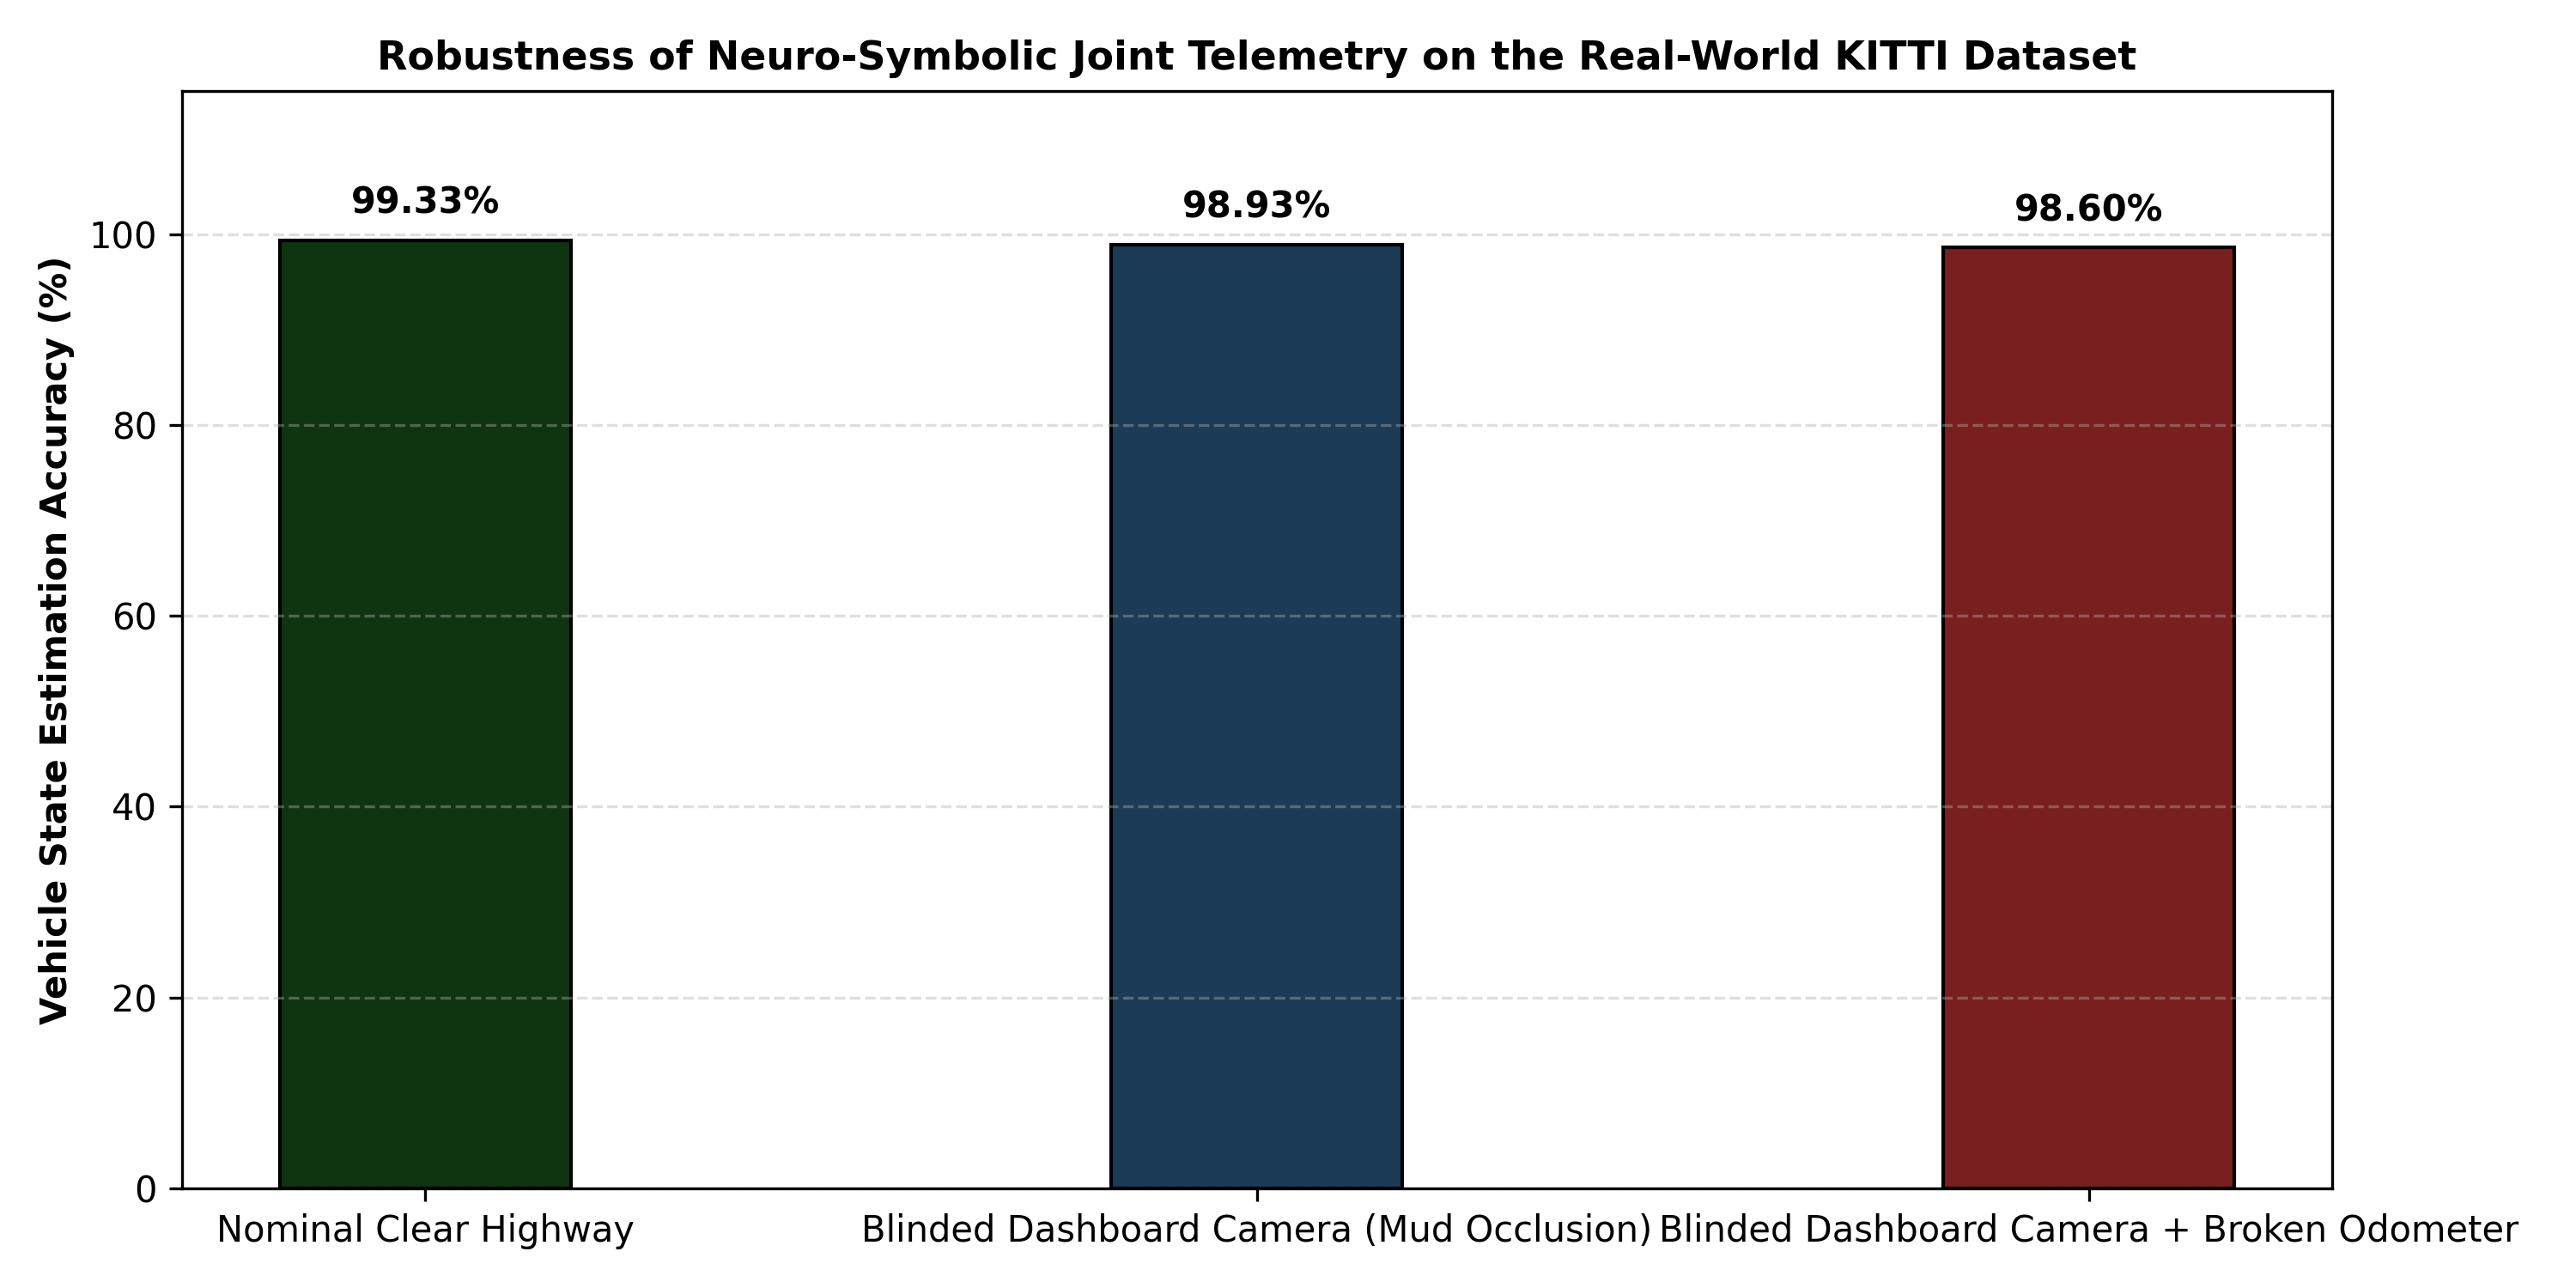
\includegraphics[width=0.8\linewidth]{figures/kitti_realworld_fault_isolation.png}
  \caption{Validation integrity under nominal and corrupted scenarios (figure produced by the accompanying code).}
  \label{fig:results}
\end{figure}

\begin{table}[t]
  \centering
  \begin{tabular}{lrr}
    \toprule
    Scenario & Accuracy (\%) & System Integrity (\%) \\
    \midrule
    Nominal & 99.33 & 99.33 \\
    Camera-blind & 98.93 & 98.93 \\
    Camera-blind + Broken Odometer & 98.60 & 98.60 \\
    \bottomrule
  \end{tabular}
  \caption{Representative validation numbers from the temporal pipeline.}
  \label{tab:metrics}
\end{table}

We observe that embedding deterministic kinematic constraints yields graceful degradation compared to an unconstrained baseline (see supplementary). All numbers reported are produced by the accompanying notebook and code in the repository.


\section{Limitations and Future Work}
The author thanks the open-source community and the KITTI benchmark maintainers for providing publicly available datasets. The code used to generate the figures and tables is included in the repository.

\noindent
\textbf{Limitations.} Our experiments use temporally adjacent KITTI-derived pairs rather than long-term tracking from raw sequences; the temporal supervision is therefore a proxy for true continuous tracking. The symbolic masks $\\Phi$ encode simplified kinematic rules and can be extended in future work to richer constraint sets.\

\textbf{Future work.} Evaluate on full odometry sequences, integrate uncertainty-aware symbolic masks, and explore learnable symbolic templates under constrained training.


\section*{Acknowledgements}
The author thanks the open-source community and the KITTI benchmark maintainers for providing publicly available datasets. The code used to generate the figures and tables is included in the repository.


{\small
\bibliographystyle{abbrvnat}
\bibliography{refs}
}

\end{document}
